
%------------------2.3 温度对反应速率的影响-----------------------
\section{温度对反应速率的影响}
\begin{frame}
	\frametitle{阿伦尼乌斯方程}
        在幂函数型速率方程中，以温度函数$f_1(T)$来体现温度对反应速率的影响。对于一定的温度，$f_1(T)$为定值，以反应速率常数$k$来表示。通常用阿伦尼乌斯方程来表示反应速率常数与温度的关系。
    \[
        k = A\exp(-E/RT) 
    \]
    式中，$A$为指前因子；$E$为活化能；$R$为气体常数。
    
    k的物理意义：所有反应组分的浓度均为1时的反应速率。
    
   
    
    化学反应速率总是随着温度的升高而增加(极少数者例外)，而且呈强烈的非线性关系。
\end{frame}


\begin{frame}
	\frametitle{阿伦尼乌斯方程的其他形式}
	微分式
	$$\frac{\mathrm{d}\ln{k}}{\mathrm{d}T} =\frac{E}{RT^2}$$
	积分式
	$$\ln{k}=\ln{A}-E/RT$$
	以$\ln{k}$对$1/T$作图可得一直线，由直线的斜率可决定反应的活化能。
	
	定积分式
	$$\ln\frac{k_2}{k_1}=\frac{-E_a}{R}(\frac{1}{T_2}-\frac{1}{T_1})$$	
\end{frame}


\begin{frame}[t]
    \frametitle{}
    \begin{question}
        可逆反应的反应速率等于正逆反应速率之差，温度升高时，可逆反应的反应速率会如何变化呢？
    \end{question}
\end{frame}


\begin{frame}
	\frametitle{正逆反应活化能的关系}
	如果可逆反应的正逆反应速率常数均符合阿伦尼乌斯方程，则有
    \[
        \frac{\mathrm{d}\ln\overrightarrow{k}}{\mathrm{d}T} =\frac{\overrightarrow{E}}{RT^2}~~~~~~~~
	\frac{\mathrm{d}\ln\overleftarrow{k}}{\mathrm{d}T} =\frac{\overleftarrow{E}}{RT^2}~~~~\Rightarrow ~~~~\frac{\mathrm{d}\ln\overrightarrow{k}}{\mathrm{d}T}-\frac{\mathrm{d}\ln\overleftarrow{k}}{\mathrm{d}T}=\frac{\overrightarrow{E}-\overleftarrow{E}}{RT^2}
    \]
	由正逆反应速率常数关系式\footnote{《反应工程》李绍芬第三版21页式2.25，$\nu$是速率控制步骤出现的次数。} \  $\overrightarrow{k}/\overleftarrow{k}=K_c^{1/\nu}$ \ 两边取对数，得$\mathrm{d}\ln\overrightarrow{k}-\mathrm{d}\ln\overleftarrow{k}=\frac{1}{\nu}\ln{K_p}$，对温度求导
	\[
        \frac{\mathrm{d}\ln\overrightarrow{k}}{\mathrm{d}T}-\frac{\mathrm{d}\ln\overleftarrow{k}}{\mathrm{d}T}=\frac{1}{\nu}\frac{\mathrm{d}\ln{K_p}}{\mathrm{d}T}
    \]
    又由范特霍夫方程$\frac{\mathrm{d}\ln{K_p}}{\mathrm{d}T}=\frac{\Delta{H_r}}{RT^2}$，则
    \[
        \overrightarrow{E}-\overleftarrow{E}=\frac{1}{\nu}\Delta{H_r}
    \]
	
    \begin{itemize}
      \item 吸热反应，$\Delta{H_r}>0$，所以$\overrightarrow{E}>\overleftarrow{E}$；
      \item 放热反应，$\Delta{H_r}<0$，$\overrightarrow{E}<\overleftarrow{E}$；
    \end{itemize}
\end{frame}


\begin{frame}
	\frametitle{正逆反应活化能的关系}
	\begin{figure}[htpb]
		\centering
		
\includegraphics[width=.9\linewidth]{活化能}
        \caption{吸热和放热反应能量示意图}
	\end{figure}
\end{frame}


\begin{frame}
	\frametitle{温度对可逆反应速率的影响}
	为方便起见，用组分A的转化率$X_A$来表示反应速率：
    \[
        r=\overrightarrow{k}f(X_A)-\overleftarrow{k}g(X_A)
    \]
	对$T$求导，得
    \[
        (\frac{\partial r}{\partial T} )_{X_A}=f({X_A})\frac{\mathrm{d}\overrightarrow{k}}{\mathrm{d}T}-g({X_A})\frac{\mathrm{d}\overleftarrow{k}}{\mathrm{d}T}
    \]
	根据阿伦尼乌斯方程\footnote{$\dif\ln\overrightarrow{x}=\frac{1}{x}\dif x$ \\ ~}
    \[
        \frac{\mathrm{d}\ln\overrightarrow{k}}{\mathrm{d}T} =\frac{\overrightarrow{E}}{RT^2}~~~~\Rightarrow~~~~\frac{\mathrm{d}\overrightarrow{k}}{\mathrm{d}T}=\frac{\overrightarrow{k}\overrightarrow{E}}{RT^2}~~~~~~~~\frac{\mathrm{d}\overleftarrow{k}}{\mathrm{d}T}=\frac{\overleftarrow{k}\overleftarrow{E}}{RT^2}
    \]
	\[
        (\frac{\partial r}{\partial T} )_{X_A}=\frac{\overrightarrow{E}}{RT^2}\overrightarrow{k}f({X_A})-\frac{\overleftarrow{E}}{RT^2}\overleftarrow{k}g({X_A})
    \]
\end{frame}


\begin{frame}
	\frametitle{温度对可逆吸热反应速率的影响}$r=\overrightarrow{k}f(X_A)-\overleftarrow{k}g(X_A)$，因为$r\ge 0$，所以$\overrightarrow{k}f({X_A})\ge \overleftarrow{k}g({X_A})$。
	\[
        (\frac{\partial r}{\partial T} )_{X_A}=\frac{\overrightarrow{E}}{RT^2}\overrightarrow{k}f({X_A})-\frac{\overleftarrow{E}}{RT^2}\overleftarrow{k}g({X_A})
    \]
    对于可逆吸热反应，$\overrightarrow{E}> \overleftarrow{E}$，$(\frac{\partial r}{\partial T} )_{X_A}> 0$

	可逆吸热反应的速率总是随着温度的升高而增加。
    \vspace{-6pt}
    \begin{figure}[htpb]
        \centering
        
\includegraphics[width=.5\linewidth]{fig2.2}
        \vspace{-7pt}
        \caption{可逆吸热反应的反应速率与温度及转化率的关系\footnote{图中曲线为等速率线。$r=0$为平衡曲线，对应平衡转化率}($r_4>r_3>r_2>r_1$)}
    \end{figure}
    \vspace{-10pt}
\end{frame}


\begin{frame}
	\frametitle{温度对可逆放热反应速率的影响}
    \begin{minipage}{0.48\linewidth}
        \[
            (\frac{\partial r}{\partial T} )_{X_A}=\frac{\overrightarrow{E}}{RT^2}\overrightarrow{k}f({X_A})-\frac{\overleftarrow{E}}{RT^2}\overleftarrow{k}g({X_A})
        \]
        对于可逆放热反应，$\overrightarrow{E}< \overleftarrow{E}$，

        但$\overrightarrow{k}f({X_A})> \overleftarrow{k}g({X_A})$，所以
        % \[
        %     > 0; (\frac{\partial r}{\partial T} )_{X_A}= 0; (\frac{\partial r}{\partial T} )_{X_A}< 0
        % \]
        \[
            (\frac{\partial r}{\partial T})_{X_A} \begin{cases}>0 \\ =0 \\ <0 \end{cases} 
        \]
    \end{minipage}\hfill
    \begin{minipage}{0.48\linewidth}
        \begin{figure}[htpb]
            \centering
            
\includegraphics[width=.8\linewidth]{fig2.3}
        \end{figure}
        
    \end{minipage}
    
    可逆放热反应的速率随着温度的升高既可能增加，又可能降低，如图所示。

    图中曲线是在一定转化率下作出的，也叫等转化率线。

	曲线的最高点$(\frac{\partial r}{\partial T})_{X_A}=0 $的温度叫做最佳温度$T_{\mathrm{op}}$。
\end{frame}


\begin{frame}
	\frametitle{可逆放热反应的最佳温度}
    \begin{minipage}{0.48\linewidth}
        反应速率极大点斜率为零，$(\frac{\partial r}{\partial T} )_{X_A}= 0$
        \[
            \overrightarrow{E}\overrightarrow{k}f({X_A})-\overleftarrow{E}\overleftarrow{k}g({X_A})=0
        \]
        \[
            \frac{\overrightarrow{E}\overrightarrow{A}\exp(-\overrightarrow{E}/RT_{\mathrm{op}})}{\overleftarrow{E}\overleftarrow{A}\exp(-\overleftarrow{E}/RT_{\mathrm{op}})}=\frac{g({X_A})}{f({X_A})}
        \]
        当反应达到平衡时，
        \[
            r=\overrightarrow{k}f(X_A)-\overleftarrow{k}g(X_A)=0
        \]
        \[
            \frac{g({X_A})}{f({X_A})}=\frac{\overrightarrow{k}}{\overleftarrow{k}}=\frac{\overrightarrow{A}\exp(-\overrightarrow{E}/RT_{\mathrm{e}})}{\overleftarrow{A}\exp(-\overleftarrow{E}/RT_{\mathrm{e}})}
        \]
    \end{minipage}\hfill
    \begin{minipage}{0.48\linewidth}
        将上式化简后两边取对数，整理后得
        \begin{framed}
        \[
            T_{\mathrm{op}}=\frac{T_{\mathrm{e}}}{1+\frac{RT_{\mathrm{e}}}{\overleftarrow{E}-\overrightarrow{E}}\ln\frac{\overleftarrow{E}}{\overrightarrow{E}}}
        \]
        \end{framed}
        \begin{itemize}
            \item 平衡温度$T_{\mathrm{e}}$是转化率的函数，故最佳温度$T_{\mathrm{op}}$是转化率的隐函数。
            \item 对应于任一转化率$X_A$，则必然有与其对应的平衡温度$T_{\mathrm{e}}$和最佳温度$T_{\mathrm{op}}$
        \end{itemize}
    \end{minipage}
\end{frame}


\begin{frame}[t]
	\frametitle{}
	\begin{block}{例2.3}
		在实际生产中合成氨反应
	$$0.5\mathrm{N_2}+1.5\mathrm{H_2}\rightleftharpoons \mathrm{NH_3}$$
	是在高温高压下采用熔融铁催化剂进行的。合成氨反应为可逆放热反应，故过程应尽可能按最佳温度曲线进行。现拟计算下列条件下的最佳温度:
	
	（1）在25.33MPa下，以3：1的氢氮混合气进行反应，氨含量为17\%；
	
	（2）其他条件同1，但氨含量为12\%；
	
	（3）把压力改为32.42MPa，其他条件同1。

	已知该催化剂的正反应活化能为$58.618\times 10^3\mathrm{J/mol}$，逆反应活化能为$\num{167.48e3}\mathrm{J/mol}$。平衡常数$K_\mathrm{p}\mathrm{(MPa^{-1})}$与温度$T$（K）及总压$p$（MPa）的关系如下：
    \[
        \lg{K_p}=(2172.26 + 19.6478p)/T – (4.2405 + 0.02149p)
    \]
	\end{block}
\end{frame}


\begin{frame}
	\frametitle{可逆放热反应最佳温度曲线}
	\begin{columns}[c]
		\column{7cm}
		\centerline{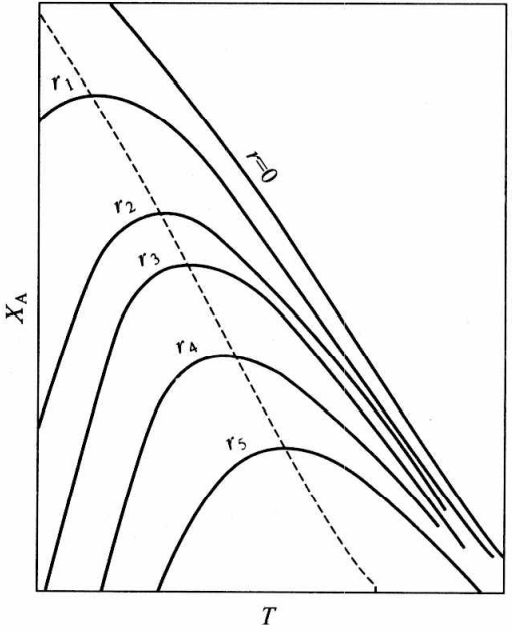
\includegraphics[width=5cm]{figs/fig2.4}}
		\centerline{\scriptsize{可逆放热反应的反应速率与温度及转化率的关系}}
		\column{7cm}
		曲线为等反应速率线，$r_5>r_4>r_3>r_2>r_1$
		\\$r=0$的曲线为平衡曲线，为反应进行的极限。
		\\连结所有等速率线上的极值点所构成的曲线(即图示虚线)，叫做最佳温度曲线。
		\\对于可逆放热反应，如果从始至终按最佳温度曲线操作，那么整个过程将以最高的反应速率进行。
	\end{columns}
\end{frame}


\begin{frame}[t]
    \frametitle{}
    \vspace{-1em}
    \begin{block}{习题2.6}
        下面是两个反应的 T-X 关系图，图中 AB 是平衡曲线 ； NP 是最佳温度曲线 ； AM 是等温线；HB 是等转化率线 。 根据下面两图回答 ：
        \begin{figure}[htpb]
            \centering
            
\includegraphics[width=.8\linewidth]{习题2.6}
        \end{figure}
        \vspace{-1em}
        \begin{enumerate}
          \item 是可逆反应还是不可逆反应？
          \item 是放热反应还是吸热反应？
        \end{enumerate}
    \end{block}
\end{frame}


\begin{frame}[t]
    \frametitle{}
    \vspace{-1em}
    \begin{block}{习题2.6}
        \begin{figure}[htpb]
            \centering
            
\includegraphics[width=.8\linewidth]{习题2.6}
        \end{figure}
        \vspace{-1em}
        \begin{enumerate}
          \item 在等温线上 ， A 、 D 、 O 、 E 、 M 点中 ， 哪点速率最大 ， 哪一点速率最小 ？
          \item 在等转化率线上 ， H 、 C 、 R 、 O 、 F 及 B 点中，哪点速率最大 ， 哪点最小 ？
          \item 在 C 、 R 两点中 ， 谁的速率大 ？
          \item 根据图中所给的十点 ， 判断哪一点速率最大 ？
        \end{enumerate}
    \end{block}
\end{frame}